\documentclass[]{article}
\usepackage{lmodern}
\usepackage{amssymb,amsmath}
\usepackage{ifxetex,ifluatex}
\usepackage{fixltx2e} % provides \textsubscript
\ifnum 0\ifxetex 1\fi\ifluatex 1\fi=0 % if pdftex
  \usepackage[T1]{fontenc}
  \usepackage[utf8]{inputenc}
\else % if luatex or xelatex
  \ifxetex
    \usepackage{mathspec}
    \usepackage{xltxtra,xunicode}
  \else
    \usepackage{fontspec}
  \fi
  \defaultfontfeatures{Mapping=tex-text,Scale=MatchLowercase}
  \newcommand{\euro}{€}
\fi
% use upquote if available, for straight quotes in verbatim environments
\IfFileExists{upquote.sty}{\usepackage{upquote}}{}
% use microtype if available
\IfFileExists{microtype.sty}{%
\usepackage{microtype}
\UseMicrotypeSet[protrusion]{basicmath} % disable protrusion for tt fonts
}{}
\ifxetex
  \usepackage[setpagesize=false, % page size defined by xetex
              unicode=false, % unicode breaks when used with xetex
              xetex]{hyperref}
\else
  \usepackage[unicode=true]{hyperref}
\fi
\usepackage[usenames,dvipsnames]{color}
\hypersetup{breaklinks=true,
            bookmarks=true,
            pdfauthor={Will Whitney},
            pdftitle={Thesis Proposal},
            colorlinks=true,
            citecolor=blue,
            urlcolor=blue,
            linkcolor=magenta,
            pdfborder={0 0 0}}
\urlstyle{same}  % don't use monospace font for urls
\usepackage{graphicx,grffile}
\makeatletter
\def\maxwidth{\ifdim\Gin@nat@width>\linewidth\linewidth\else\Gin@nat@width\fi}
\def\maxheight{\ifdim\Gin@nat@height>\textheight\textheight\else\Gin@nat@height\fi}
\makeatother
% Scale images if necessary, so that they will not overflow the page
% margins by default, and it is still possible to overwrite the defaults
% using explicit options in \includegraphics[width, height, ...]{}
\setkeys{Gin}{width=\maxwidth,height=\maxheight,keepaspectratio}
\setlength{\parindent}{0pt}
\setlength{\parskip}{6pt plus 2pt minus 1pt}
\setlength{\emergencystretch}{3em}  % prevent overfull lines
\providecommand{\tightlist}{%
  \setlength{\itemsep}{0pt}\setlength{\parskip}{0pt}}
\setcounter{secnumdepth}{5}

\title{Thesis Proposal}
\author{Will Whitney}
\date{}
\usepackage{simple}
\AtBeginDocument{%
\renewcommand*\figurename{Figure}
\renewcommand*\tablename{Table}
}
\AtBeginDocument{%
\renewcommand*\listfigurename{List of Figures}
\renewcommand*\listtablename{List of Tables}
}
\usepackage{float}
\floatstyle{ruled}
\makeatletter
\@ifundefined{c@chapter}{\newfloat{codelisting}{h}{lop}}{\newfloat{codelisting}{h}{lop}[chapter]}
\makeatother
\floatname{codelisting}{Listing}
\newcommand*\listoflistings{\listof{codelisting}{List of Listings}}

% Redefines (sub)paragraphs to behave more like sections
\ifx\paragraph\undefined\else
\let\oldparagraph\paragraph
\renewcommand{\paragraph}[1]{\oldparagraph{#1}\mbox{}}
\fi
\ifx\subparagraph\undefined\else
\let\oldsubparagraph\subparagraph
\renewcommand{\subparagraph}[1]{\oldsubparagraph{#1}\mbox{}}
\fi

\begin{document}
\maketitle

\section{Introduction}\label{introduction}

A defining feature of human intelligence is the ability to apply
knowledge and techniques learned on one problem to other problems which
have similar components. This ranges from the simplest examples
(e.g.~playing chess with different-colored pieces than you learned with)
to the most complicated (like applying concepts from one domain of
mathematics to another). A particular formulation of these problems is
referred to as transfer learning.

To date, machine learning algorithms have struggled with transfer
learning tasks. In some cases existing techniques perform so poorly as
to exhibit ``negative transfer'', in which seeing examples across new
domains causes the learner to perform worse than it did before (Pan \&
Yang, 2010).

With the recent success of deep learning methods in many fields, efforts
have been made to apply deep learning techniques to transfer learning
problems. Deep learning is at the deepest level a method for
hierarchically extracting good representations from complex data, with
the higher levels of a network capturing increasingly abstract
representations of the data. As such, deep learning seems naively to be
a promising direction for transfer learning; abstract representations of
the data should be useful for many related tasks, and the network should
be able to simply not use any which are not helpful.

\subsection{Catastrophic forgetting}\label{catastrophic-forgetting}

This theory has been borne out for simple, highly coupled tasks such as
evaluating sentiment of reviews for different categories of products
(Glorot, Bordes, \& Bengio, 2011). A more wide-ranging survey of deep
learning methods for transfer learning shows that some classes of models
are able to improve their performance on the original, clean dataset
after being shown perturbed or distorted versions of the same data
(Bengio, 2012).

However, even small changes in the task result in substantial changes to
the optimal features, especially at high levels of the network
(Yosinski, Clune, Bengio, \& Lipson, 2014). This can lead to
\emph{catastrophic forgetting}, in which the network ``unlearns'' its
original task as it trains on a new one. A recent set of experiments
(Goodfellow, Mirza, Xiao, Courville, \& Bengio, 2013) detail the
tradeoff curve for performance on one task versus performance on the
other task for both similar and dissimilar tasks. They show that for
networks trained on two tasks, improvement on one task comes at a cost
to performance on another.

The true goal of such a system should be \emph{function reuse}. Ideally
a system for transfer learning would learn a set of distinct functions
which it uses to solve a given domain of tasks. Each of these functions
would represent a particular transformation of the data relevant to
solving the problem. Then when presented with a new domain of tasks,
this system would have those functions available and could choose
whether or not to use them as appropriate for a given task in the new
domain. This reuse would represent shared structure between the two
domains.

To achieve this, it will be necessary to draw on recent work in
attentional models.

\subsection{Attentional models}\label{attentional-models}

Recently a very powerful new class of neural networks known as
attentional models have shown success on a variety of difficult tasks.
The Neural Turing Machine (Graves, Wayne, \& Danihelka, 2014) (NTM)
performs complex operations on sequences such as sorting or repeatedly
copying by using a differentiable addressing mechanism to read and write
to an external memory. DRAW (Gregor, Danihelka, Graves, \& Wierstra,
2015) uses a differentiable attention system to selectively read from
its input image and write to an output canvas, as shown in
Fig.~\ref{fig:draw}.

\begin{figure}[htbp]
\centering
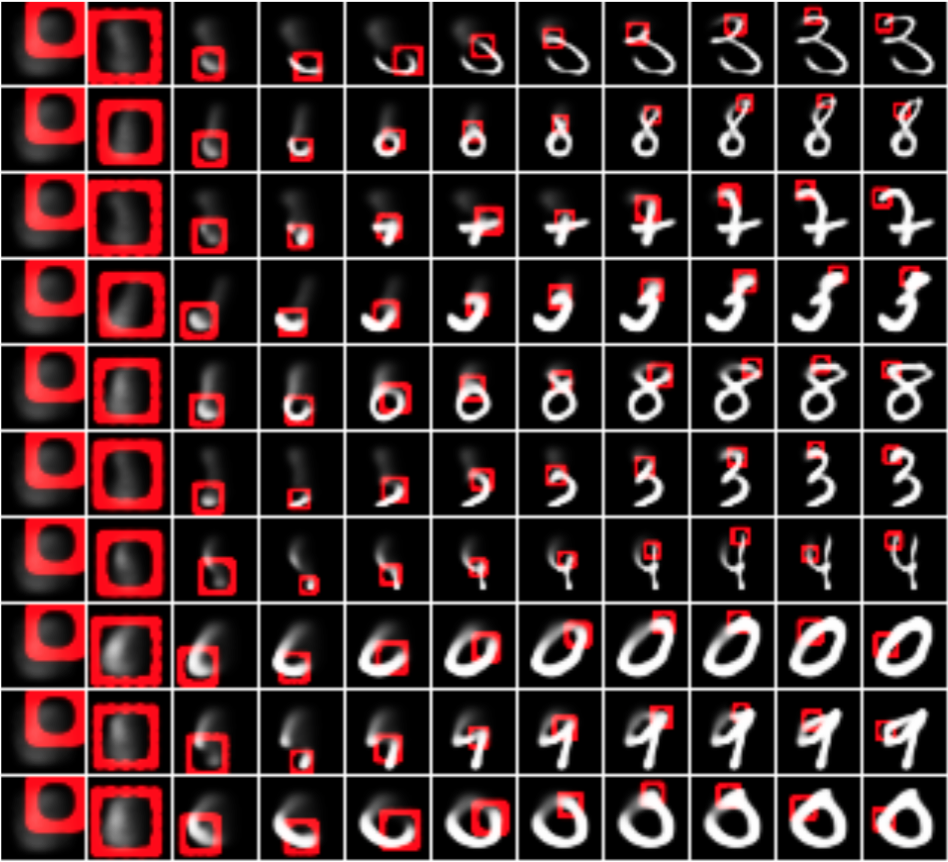
\includegraphics{draw_attention_small.png}
\caption{\label{fig:draw}The DRAW network uses attention to render
digits onto a canvas.}
\end{figure}

These systems work by having a Long Short-Term Memory (Hochreiter \&
Schmidhuber, 1997) (LSTM) controller which produces a weighting
distribution over the cells of data structure it indexes. This weighting
for each cell is, with some variations in each system, multiplied by the
content of the cell and then summed across cells (when reading) or
multiplied by the value to write and then added into the cell (when
writing).

This attention system allows the network to sequentially

\begin{enumerate}
\def\labelenumi{\arabic{enumi}.}
\tightlist
\item
  Decide on a region of the data to focus on, then
\item
  Read or edit just that region of the data.
\end{enumerate}

By letting the network sequentially attend to a particular region of the
input, this design gives a small attentional network the same power as
an enormous one with fixed connectivity. Furthermore, since such a
system can decide from one timestep to the next what part of the data is
the most important, it can effectively ignore the less diagnostic
components of an input or output (e.g., never look at the background of
an image).

In this paper, the author proposes a model for transfer learning which
addresses the challenge of reusing whichever subroutines are shared
between several different tasks without forgetting those subroutines the
tasks do not have in common. The proposed system takes the form of an
attentional model over components of the network itself.

\section{Model}\label{model}

\begin{figure}[htbp]
\centering
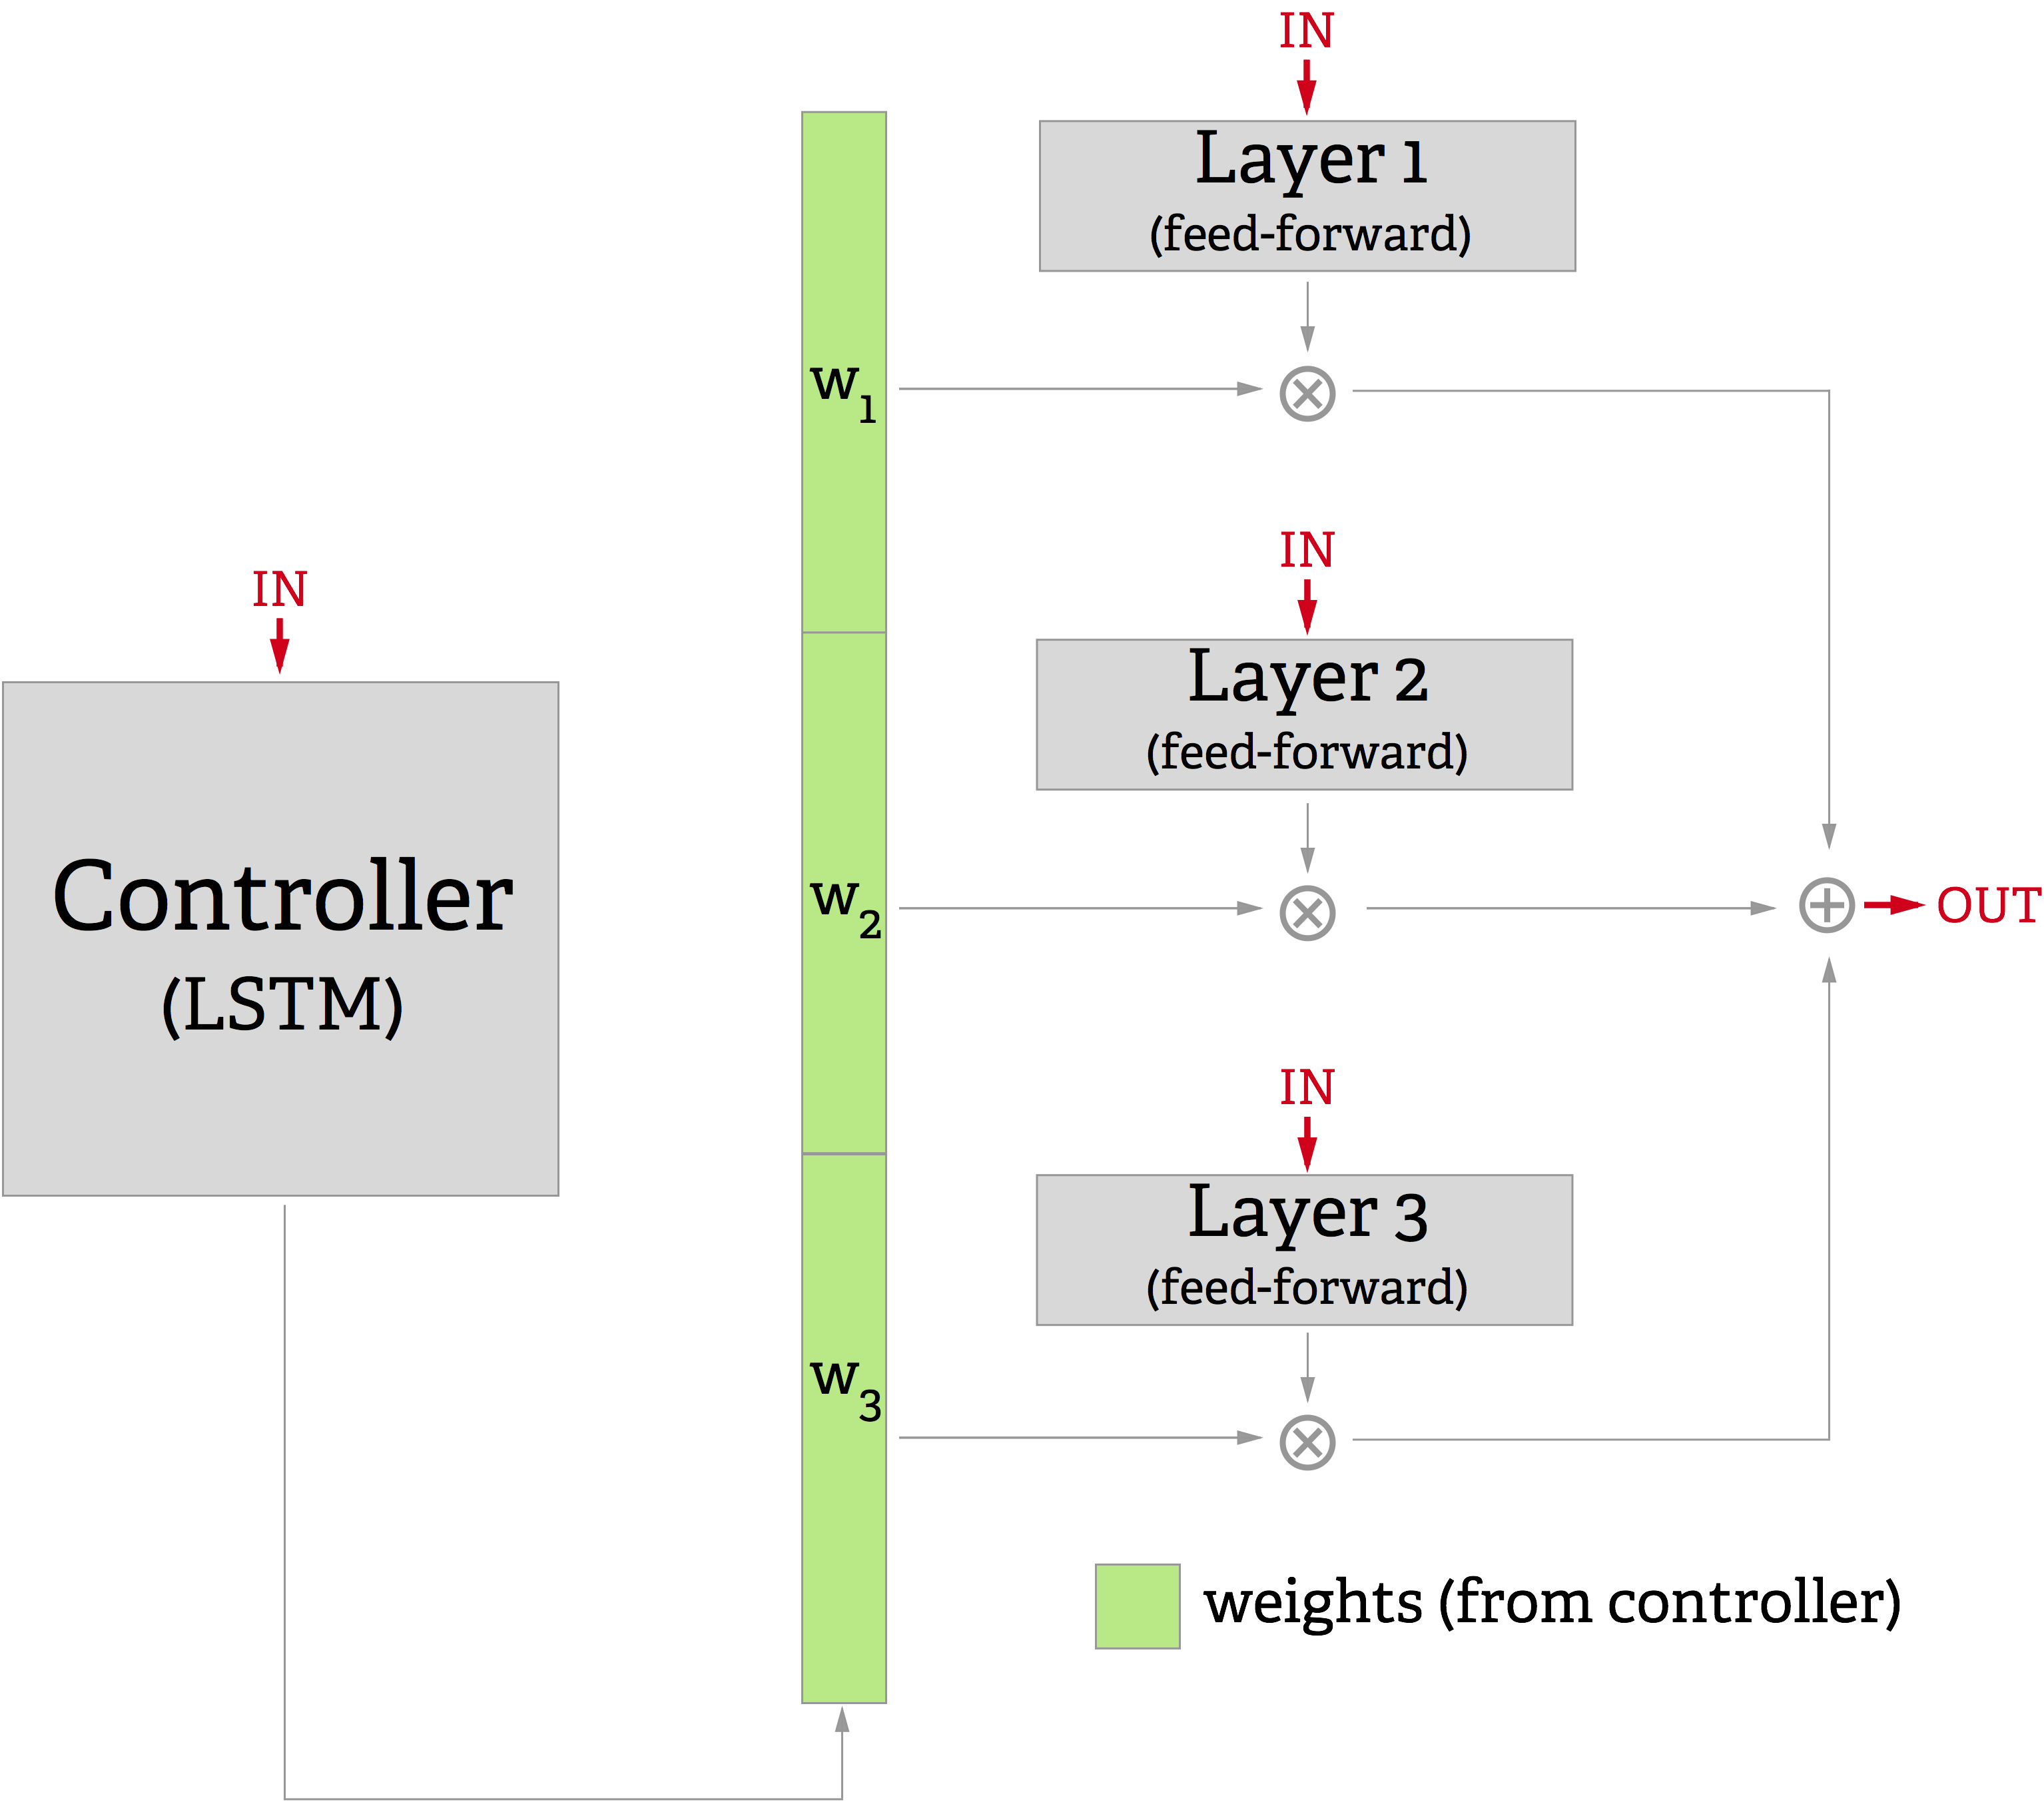
\includegraphics{controller_network_small.png}
\caption{\label{fig:controller_network}The controller and layers of the
system. The controller provides weights on each layer as a function of
the data. This shows three layers, but there can be many more.}
\end{figure}

The proposed model generates an output for a particular timestep via the
following steps (shown in Fig.~\ref{fig:controller_network}):

\begin{enumerate}
\def\labelenumi{\arabic{enumi}.}
\tightlist
\item
  The input tensor is fed into the controller
\item
  The controller decides which layers are most appropriate for
  processing this input
\item
  The controller outputs a weighting vector reflecting how much output
  it wants from each of the layers
\item
  The input tensor is fed into each layer (in parallel)
\item
  The outputs from each layer are multiplied by their respective weights
  from the controller
\item
  The weighted outputs from all the layers are summed together and
  output. This is the output of the whole network for this timestep.
\end{enumerate}

Essentially the idea is that at each timestep, the controller examines
the input that it gets, then up- or down-regulates the activities of the
various ``functions'' (single-layer NNs) to best deal with this input.
Since the controller is an LSTM, it can store information about the
inputs it has received before, meaning that in a time series or language
setting it can make weighting decisions contextually.

As this model is differentiable throughout, it can be trained with the
standard backpropagation through time (BPTT) algorithm for stochastic
gradient descent.

By setting weights over each of the layers in the network, the
controller scales not only the output of each layer, but also the error
gradient that it receives. This means that in a given timestep, the
layers which have very low weights on their output will be nearly
unchanged by the learning process. That is, functions which are not used
are not forgotten.

In an ordinary feedforward neural network, the only way for the network
to prevent learning in a particular node is for it to learn connection
strengths very near zero for that node. This takes many training
examples, and functionally removes that node from the computation graph.

This system, by comparison, can decide that a set of nodes is or is not
relevant on an input-by-input basis.

\subsection{Multi-step variant}\label{multi-step-variant}

\begin{figure}[htbp]
\centering
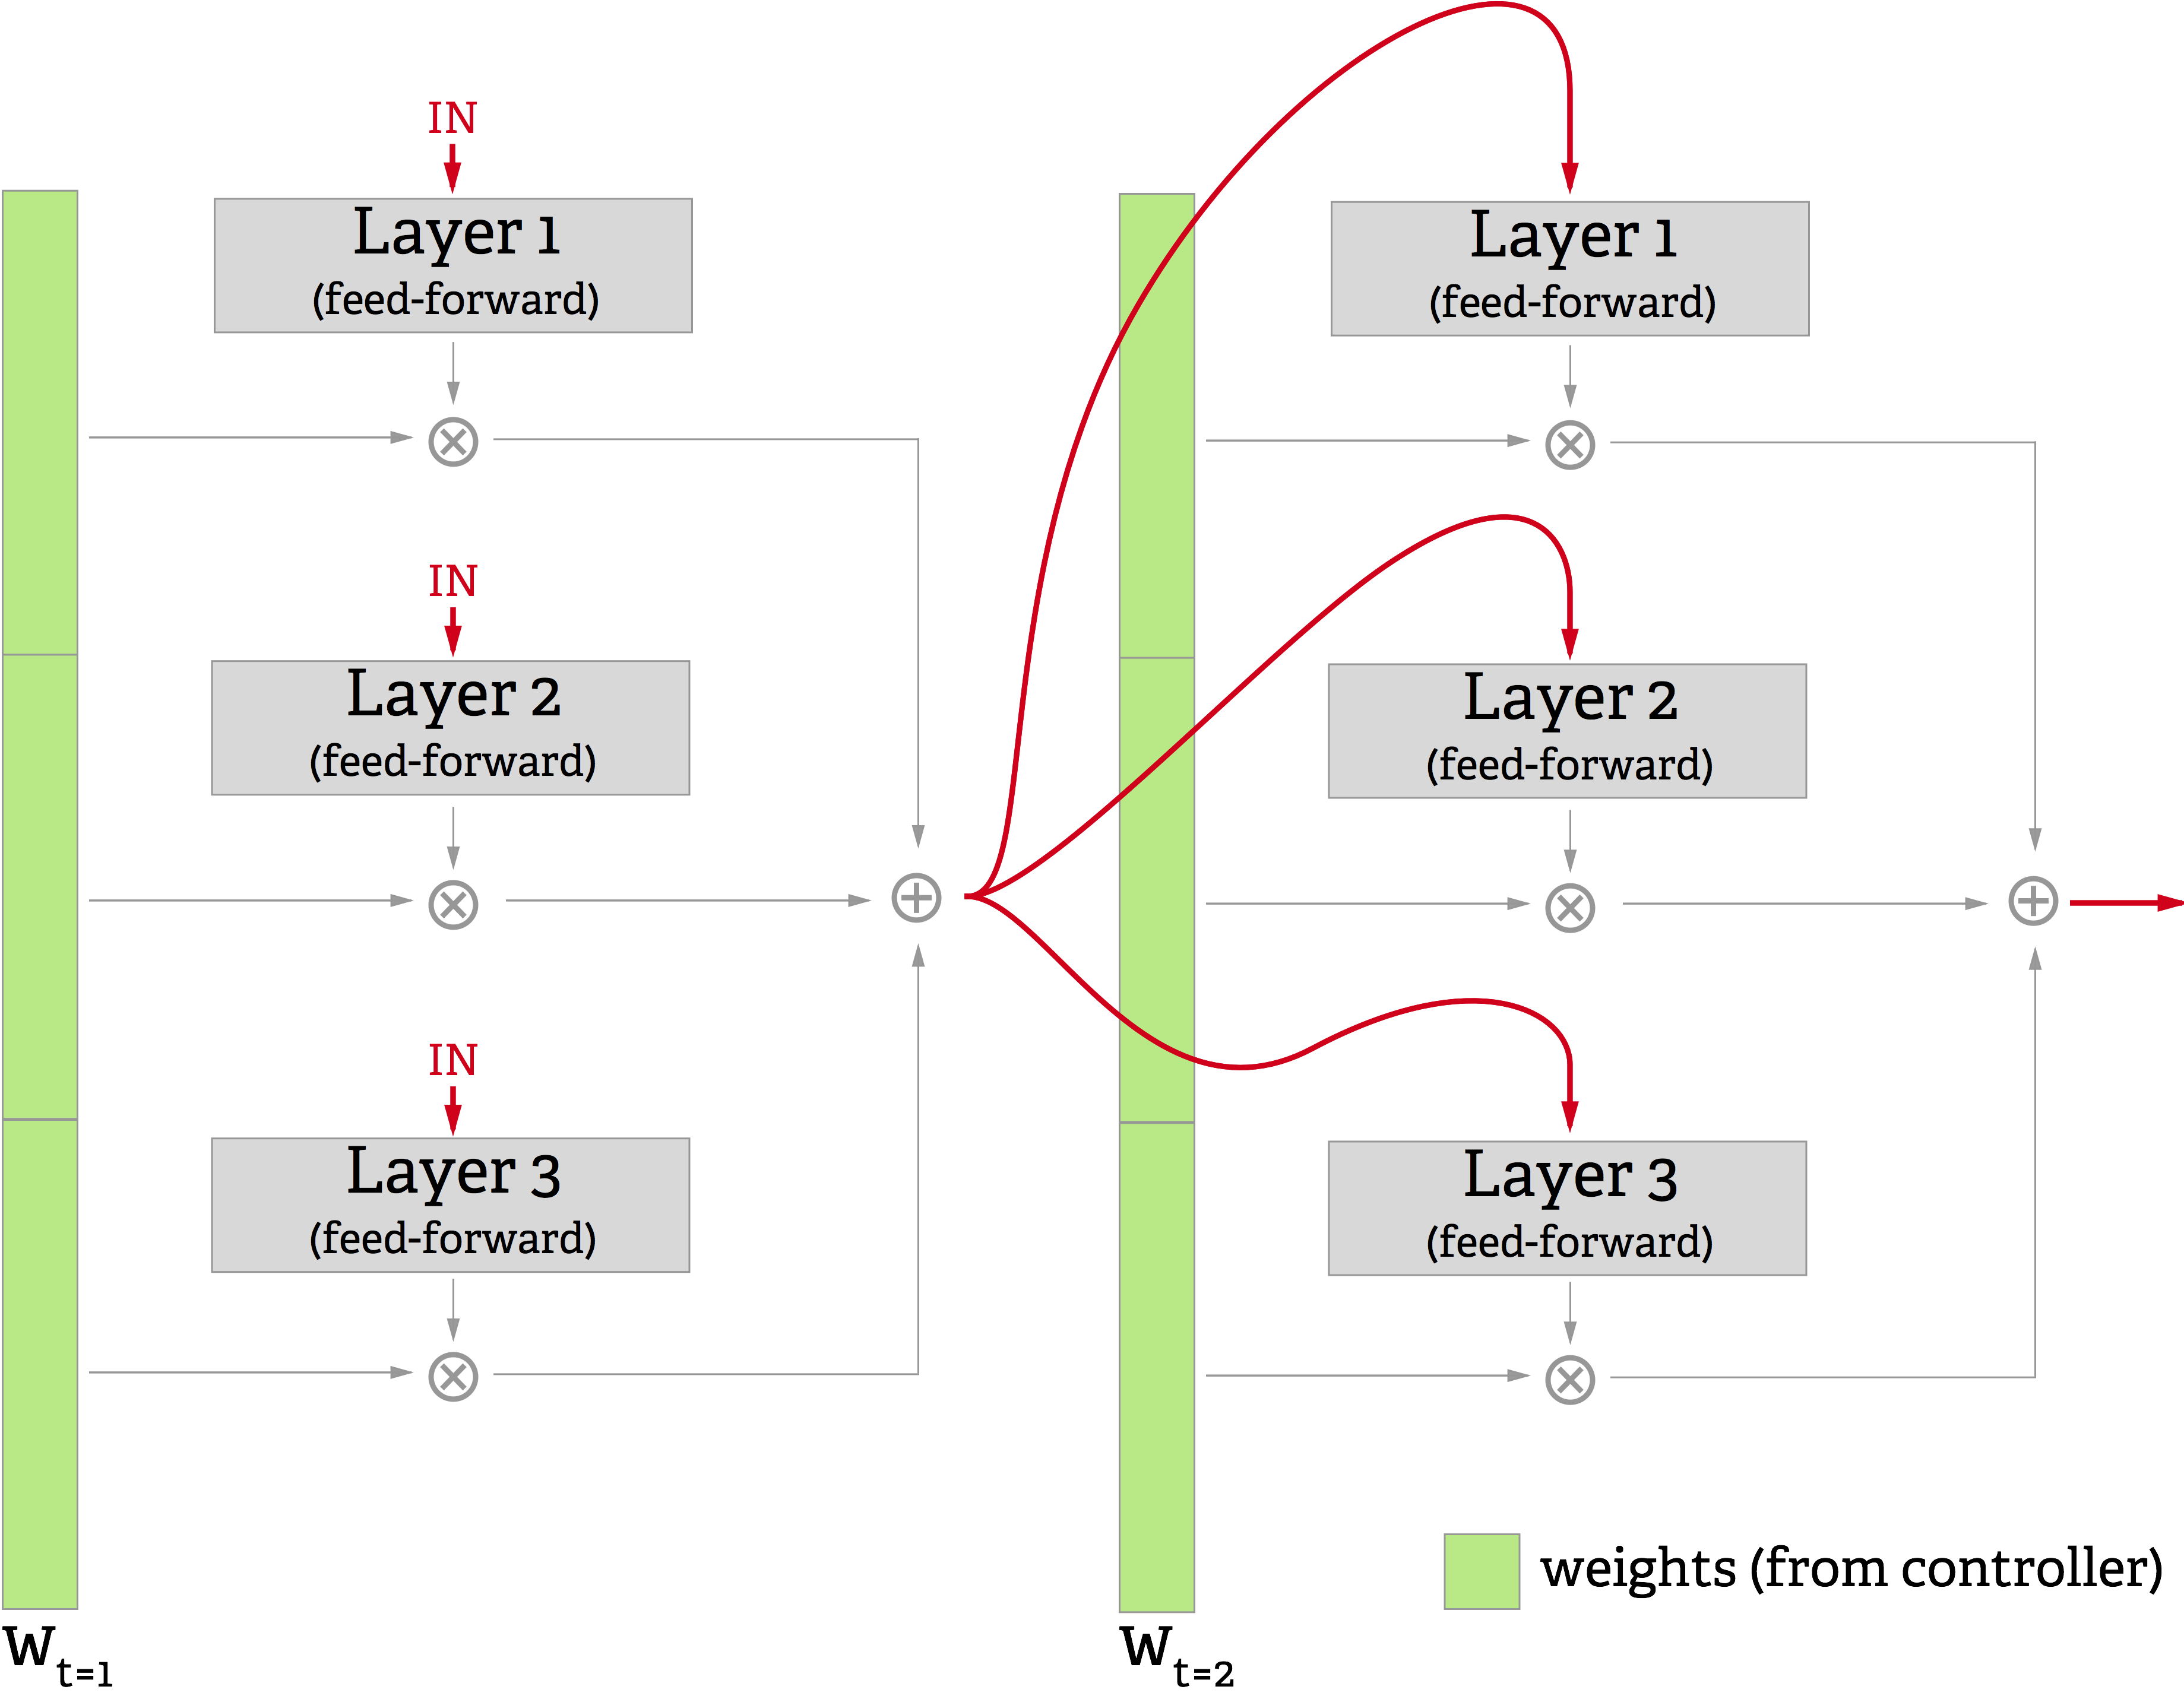
\includegraphics{multistep_small.png}
\caption{\label{fig:multistep}A variant of the design for using multiple
timesteps (in this case, two) to calculate each output.}
\end{figure}

One obvious question to consider about this model is, ``What happens if
the correct output function at a timestep is not computable with a
linear combination of single-layer networks?'' After all, there are
functions computable by a polynomial-width network of depth \texttt{k}
that require exponential width to compute with a network of depth
\texttt{k-1} (Hastad, 1986).

To address this question, the system could be run for a predefined
number of steps between outputs. That is,

\begin{enumerate}
\def\labelenumi{\arabic{enumi}.}
\tightlist
\item
  Feed the system the input for ``real-world'' time \texttt{t} and save
  the output
\item
  Repeat \texttt{k} times:

  \begin{enumerate}
  \def\labelenumii{\alph{enumii}.}
  \tightlist
  \item
    Feed the system its own most recent output
  \end{enumerate}
\item
  Take the \texttt{kth} output of the system as its answer for time
  \texttt{t}
\item
  Repeat from 1. for time \texttt{t+1}
\end{enumerate}

This amounts to making the network deeper, in that more layers of
computation and nonlinearity lie between the input and the output. This
gives it the same computational power of a \texttt{k}-depth model.

\subsection{Function reuse}\label{function-reuse}

The fundamental problem this model attempts to address is that of
\emph{function reuse}. Given that two tasks require some of the same
computation to solve, can we build a system that only has to learn that
computation once?

If this system has learned a function in one task which happens to also
solve another task, the error gradients propagated to the controller
will consistently increase the weight assigned to that function and
decrease that assigned to the other functions. But this depends on a
particular subroutine of one task being exactly the solution to another.

One result which provides hope for partial function reuse is given by
Yosinski et al. (2014), who showed that a deep network trained to
recognize one domain of objects learned to recognize a new domain of
objects far faster than an untrained, randomly-initialized network. So
clearly there are domains with substantial overlap in their subroutines.

In order to encourage this behavior, it may be necessary to train the
network on multiple domains simultaneously, thus letting the functions
``coevolve'' on all domains and encouraging separation of shared
resources from those that are domain-specific.

Whether or not this happens in practice in an experimental question, but
the proposed model provides a framework in which it is possible.

\subsection{Connections to mixture of
experts}\label{connections-to-mixture-of-experts}

This architecture has connections to the mixture of experts model
proposed by Jacobs et al. (1991), in which several different
task-specific ``expert'' networks each contribute in linear combination
to the output of the overall network. The model proposed in this paper
can be thought of as akin to an ``iterated mixture of experts'', in
which a mixture of experts model is sequentially applied to its own
output several times before a final output from the network is produced.

However, this model has two key differences from this ``iterated mixture
of experts'':

\begin{enumerate}
\def\labelenumi{\arabic{enumi}.}
\tightlist
\item
  \textbf{The gating network is an LSTM.} This means that the gating
  network (or controller, in my terminology) can easily learn fixed
  sequential procedures for certain types of input.
\item
  \textbf{The ``expert'' networks are extremely simple.} Because the
  model has memory and is iterated, the expert networks are made as
  simple as they can be: single layers. This give the controller as much
  flexibility as possible about how to compose functions instead of just
  choosing between them.
\end{enumerate}

\section{Experiments}\label{experiments}

\subsection{Games}\label{games}

One compelling domain for transfer learning is simple arcade games such
as Pac-Man or Breakout. Models such as the DQN (Mnih et al., 2015) have
been recently shown to perform very well on a subset of these games when
trained for one game only, but so far efforts to play multiple games
with one network have failed. Even minor perturbations in the visual
representation of a game (e.g.~changing the colors) require substantial
retraining.

The author proposes to test the transfer learning abilities of this
system by training it with interleaved examples of two similar games at
a time. Pairs of games with different levels of similarity can be
constructed by everything from creating minor visual differences in the
same game to using different source games (e.g.~Breakout versus Space
Invaders).

Additionally, it would be interesting to see whether the system can
efficiently perform curriculum learning. Curriculum learning is a subset
of transfer learning which involves transferring skills learned on easy
problems in a domain to harder problems in the same domain. Puzzle games
with levels of increasing difficulty, such as Rush Hour, would be an
interesting domain for this.

\section{Discussion}\label{discussion}

This paper proposes a system capable of taking on challenges in the
domain of transfer learning using a model of functional attention. This
model consists of an LSTM controller which allots attention and a set of
layers which learn functions. By separating the decision of \emph{what
to execute} from the \emph{execution}, this model will prevent the
problems of catastrophic forgetting and negative transfer while allowing
the reuse of subcomputations which are shared between tasks.

\section*{References}\label{references}
\addcontentsline{toc}{section}{References}

Bengio, Y. (2012). Deep learning of representations for unsupervised and
transfer learning. \emph{Unsupervised and Transfer Learning Challenges
in Machine Learning}, \emph{7}, 19.

Glorot, X., Bordes, A., \& Bengio, Y. (2011). Domain adaptation for
large-scale sentiment classification: A deep learning approach. In
\emph{Proceedings of the 28th international conference on machine
learning (iCML-11)} (pp. 513--520).

Goodfellow, I. J., Mirza, M., Xiao, D., Courville, A., \& Bengio, Y.
(2013). An empirical investigation of catastrophic forgeting in
gradient-based neural networks. \emph{ArXiv Preprint ArXiv:1312.6211}.

Graves, A., Wayne, G., \& Danihelka, I. (2014). Neural turing machines.
\emph{ArXiv Preprint ArXiv:1410.5401}.

Gregor, K., Danihelka, I., Graves, A., \& Wierstra, D. (2015). DRAW: A
recurrent neural network for image generation. \emph{ArXiv Preprint
ArXiv:1502.04623}.

Hastad, J. (1986). Almost optimal lower bounds for small depth circuits.
In \emph{Proceedings of the eighteenth annual aCM symposium on theory of
computing} (pp. 6--20). ACM.

Hochreiter, S., \& Schmidhuber, J. (1997). Long short-term memory.
\emph{Neural Computation}, \emph{9}(8), 1735--1780.

Jacobs, R. A., Jordan, M. I., \& Barto, A. G. (1991). Task decomposition
through competition in a modular connectionist architecture: The what
and where vision tasks. \emph{Cognitive Science}, \emph{15}(2),
219--250.

Mnih, V., Kavukcuoglu, K., Silver, D., Rusu, A. A., Veness, J.,
Bellemare, M. G., \ldots{} others. (2015). Human-level control through
deep reinforcement learning. \emph{Nature}, \emph{518}(7540), 529--533.

Pan, S. J., \& Yang, Q. (2010). A survey on transfer learning.
\emph{Knowledge and Data Engineering, IEEE Transactions on},
\emph{22}(10), 1345--1359.

Yosinski, J., Clune, J., Bengio, Y., \& Lipson, H. (2014). How
transferable are features in deep neural networks? In \emph{Advances in
neural information processing systems} (pp. 3320--3328).

\end{document}
